% Options for packages loaded elsewhere
\PassOptionsToPackage{unicode}{hyperref}
\PassOptionsToPackage{hyphens}{url}
%
\documentclass[
]{article}
\usepackage{amsmath,amssymb}
\usepackage{lmodern}
\usepackage{iftex}
\ifPDFTeX
  \usepackage[T1]{fontenc}
  \usepackage[utf8]{inputenc}
  \usepackage{textcomp} % provide euro and other symbols
\else % if luatex or xetex
  \usepackage{unicode-math}
  \defaultfontfeatures{Scale=MatchLowercase}
  \defaultfontfeatures[\rmfamily]{Ligatures=TeX,Scale=1}
\fi
% Use upquote if available, for straight quotes in verbatim environments
\IfFileExists{upquote.sty}{\usepackage{upquote}}{}
\IfFileExists{microtype.sty}{% use microtype if available
  \usepackage[]{microtype}
  \UseMicrotypeSet[protrusion]{basicmath} % disable protrusion for tt fonts
}{}
\makeatletter
\@ifundefined{KOMAClassName}{% if non-KOMA class
  \IfFileExists{parskip.sty}{%
    \usepackage{parskip}
  }{% else
    \setlength{\parindent}{0pt}
    \setlength{\parskip}{6pt plus 2pt minus 1pt}}
}{% if KOMA class
  \KOMAoptions{parskip=half}}
\makeatother
\usepackage{xcolor}
\usepackage[margin=1in]{geometry}
\usepackage{color}
\usepackage{fancyvrb}
\newcommand{\VerbBar}{|}
\newcommand{\VERB}{\Verb[commandchars=\\\{\}]}
\DefineVerbatimEnvironment{Highlighting}{Verbatim}{commandchars=\\\{\}}
% Add ',fontsize=\small' for more characters per line
\usepackage{framed}
\definecolor{shadecolor}{RGB}{248,248,248}
\newenvironment{Shaded}{\begin{snugshade}}{\end{snugshade}}
\newcommand{\AlertTok}[1]{\textcolor[rgb]{0.94,0.16,0.16}{#1}}
\newcommand{\AnnotationTok}[1]{\textcolor[rgb]{0.56,0.35,0.01}{\textbf{\textit{#1}}}}
\newcommand{\AttributeTok}[1]{\textcolor[rgb]{0.77,0.63,0.00}{#1}}
\newcommand{\BaseNTok}[1]{\textcolor[rgb]{0.00,0.00,0.81}{#1}}
\newcommand{\BuiltInTok}[1]{#1}
\newcommand{\CharTok}[1]{\textcolor[rgb]{0.31,0.60,0.02}{#1}}
\newcommand{\CommentTok}[1]{\textcolor[rgb]{0.56,0.35,0.01}{\textit{#1}}}
\newcommand{\CommentVarTok}[1]{\textcolor[rgb]{0.56,0.35,0.01}{\textbf{\textit{#1}}}}
\newcommand{\ConstantTok}[1]{\textcolor[rgb]{0.00,0.00,0.00}{#1}}
\newcommand{\ControlFlowTok}[1]{\textcolor[rgb]{0.13,0.29,0.53}{\textbf{#1}}}
\newcommand{\DataTypeTok}[1]{\textcolor[rgb]{0.13,0.29,0.53}{#1}}
\newcommand{\DecValTok}[1]{\textcolor[rgb]{0.00,0.00,0.81}{#1}}
\newcommand{\DocumentationTok}[1]{\textcolor[rgb]{0.56,0.35,0.01}{\textbf{\textit{#1}}}}
\newcommand{\ErrorTok}[1]{\textcolor[rgb]{0.64,0.00,0.00}{\textbf{#1}}}
\newcommand{\ExtensionTok}[1]{#1}
\newcommand{\FloatTok}[1]{\textcolor[rgb]{0.00,0.00,0.81}{#1}}
\newcommand{\FunctionTok}[1]{\textcolor[rgb]{0.00,0.00,0.00}{#1}}
\newcommand{\ImportTok}[1]{#1}
\newcommand{\InformationTok}[1]{\textcolor[rgb]{0.56,0.35,0.01}{\textbf{\textit{#1}}}}
\newcommand{\KeywordTok}[1]{\textcolor[rgb]{0.13,0.29,0.53}{\textbf{#1}}}
\newcommand{\NormalTok}[1]{#1}
\newcommand{\OperatorTok}[1]{\textcolor[rgb]{0.81,0.36,0.00}{\textbf{#1}}}
\newcommand{\OtherTok}[1]{\textcolor[rgb]{0.56,0.35,0.01}{#1}}
\newcommand{\PreprocessorTok}[1]{\textcolor[rgb]{0.56,0.35,0.01}{\textit{#1}}}
\newcommand{\RegionMarkerTok}[1]{#1}
\newcommand{\SpecialCharTok}[1]{\textcolor[rgb]{0.00,0.00,0.00}{#1}}
\newcommand{\SpecialStringTok}[1]{\textcolor[rgb]{0.31,0.60,0.02}{#1}}
\newcommand{\StringTok}[1]{\textcolor[rgb]{0.31,0.60,0.02}{#1}}
\newcommand{\VariableTok}[1]{\textcolor[rgb]{0.00,0.00,0.00}{#1}}
\newcommand{\VerbatimStringTok}[1]{\textcolor[rgb]{0.31,0.60,0.02}{#1}}
\newcommand{\WarningTok}[1]{\textcolor[rgb]{0.56,0.35,0.01}{\textbf{\textit{#1}}}}
\usepackage{graphicx}
\makeatletter
\def\maxwidth{\ifdim\Gin@nat@width>\linewidth\linewidth\else\Gin@nat@width\fi}
\def\maxheight{\ifdim\Gin@nat@height>\textheight\textheight\else\Gin@nat@height\fi}
\makeatother
% Scale images if necessary, so that they will not overflow the page
% margins by default, and it is still possible to overwrite the defaults
% using explicit options in \includegraphics[width, height, ...]{}
\setkeys{Gin}{width=\maxwidth,height=\maxheight,keepaspectratio}
% Set default figure placement to htbp
\makeatletter
\def\fps@figure{htbp}
\makeatother
\setlength{\emergencystretch}{3em} % prevent overfull lines
\providecommand{\tightlist}{%
  \setlength{\itemsep}{0pt}\setlength{\parskip}{0pt}}
\setcounter{secnumdepth}{-\maxdimen} % remove section numbering
\ifLuaTeX
  \usepackage{selnolig}  % disable illegal ligatures
\fi
\IfFileExists{bookmark.sty}{\usepackage{bookmark}}{\usepackage{hyperref}}
\IfFileExists{xurl.sty}{\usepackage{xurl}}{} % add URL line breaks if available
\urlstyle{same} % disable monospaced font for URLs
\hypersetup{
  pdftitle={aflevering},
  hidelinks,
  pdfcreator={LaTeX via pandoc}}

\title{aflevering}
\author{}
\date{\vspace{-2.5em}2023-10-17}

\begin{document}
\maketitle

\hypertarget{r-markdown}{%
\subsection{R Markdown}\label{r-markdown}}

\begin{Shaded}
\begin{Highlighting}[]
\FunctionTok{load}\NormalTok{(}\StringTok{"DWBdata.Rdata"}\NormalTok{)}
\NormalTok{fit1 }\OtherTok{\textless{}{-}} \FunctionTok{lmer}\NormalTok{(DWB100 }\SpecialCharTok{\textasciitilde{}}\NormalTok{ WkDay }\SpecialCharTok{+}\NormalTok{ z2sleep }\SpecialCharTok{+}\NormalTok{ (z2sleep}\SpecialCharTok{|}\NormalTok{NameID), }\AttributeTok{data =}\NormalTok{ DWBdata)}
\FunctionTok{fixef}\NormalTok{(fit1)}
\end{Highlighting}
\end{Shaded}

\begin{verbatim}
## (Intercept)      WkDay2      WkDay3      WkDay4      WkDay5      WkDay6 
##  56.7802389  -0.2664728  -0.9063820  -1.5689017  -1.5536840   2.9100872 
##      WkDay7     z2sleep 
##   2.7232162   7.2078672
\end{verbatim}

\begin{Shaded}
\begin{Highlighting}[]
\CommentTok{\# t distribution with 3 degrees of freedom}

\NormalTok{fit2 }\OtherTok{\textless{}{-}} \FunctionTok{lmer}\NormalTok{(DWB100 }\SpecialCharTok{\textasciitilde{}}\NormalTok{ WkDay }\SpecialCharTok{+}\NormalTok{ z2sleep }\SpecialCharTok{+}\NormalTok{ (}\DecValTok{1}\SpecialCharTok{|}\NormalTok{NameID), }\AttributeTok{data =}\NormalTok{ DWBdata)}
\NormalTok{M }\OtherTok{\textless{}{-}} \FloatTok{2e3}
\NormalTok{X }\OtherTok{\textless{}{-}}\NormalTok{ fit2 }\SpecialCharTok{\%\textgreater{}\%} \FunctionTok{model.matrix}\NormalTok{()}
\NormalTok{Z }\OtherTok{\textless{}{-}}\NormalTok{ fit2 }\SpecialCharTok{\%\textgreater{}\%} \FunctionTok{getME}\NormalTok{(}\AttributeTok{name=}\StringTok{"Z"}\NormalTok{)}
\NormalTok{beta }\OtherTok{\textless{}{-}} \FunctionTok{fixef}\NormalTok{(fit2)}
\NormalTok{tau }\OtherTok{\textless{}{-}}\NormalTok{ (}\FunctionTok{VarCorr}\NormalTok{(fit2) }\SpecialCharTok{\%\textgreater{}\%} \FunctionTok{as.data.frame}\NormalTok{())}\SpecialCharTok{$}\NormalTok{sdcor[}\DecValTok{1}\NormalTok{]}
\NormalTok{sigma }\OtherTok{\textless{}{-}}\NormalTok{ (}\FunctionTok{VarCorr}\NormalTok{(fit2) }\SpecialCharTok{\%\textgreater{}\%} \FunctionTok{as.data.frame}\NormalTok{())}\SpecialCharTok{$}\NormalTok{sdcor[}\DecValTok{2}\NormalTok{]}
\NormalTok{resMat }\OtherTok{\textless{}{-}} \FunctionTok{matrix}\NormalTok{(}\ConstantTok{NA}\NormalTok{,M,}\DecValTok{3}\NormalTok{)}
\ControlFlowTok{for}\NormalTok{ (i }\ControlFlowTok{in} \DecValTok{1}\SpecialCharTok{:}\NormalTok{M) \{}
\NormalTok{B }\OtherTok{\textless{}{-}} \FunctionTok{rt}\NormalTok{(}\DecValTok{27}\NormalTok{, }\DecValTok{3}\NormalTok{)}\SpecialCharTok{*}\NormalTok{tau}\SpecialCharTok{/}\NormalTok{(}\FunctionTok{sqrt}\NormalTok{(}\DecValTok{3}\SpecialCharTok{/}\NormalTok{(}\DecValTok{3{-}2}\NormalTok{)))}
\NormalTok{eps }\OtherTok{\textless{}{-}} \FunctionTok{rnorm}\NormalTok{(}\FunctionTok{nrow}\NormalTok{(DWBdata), }\DecValTok{0}\NormalTok{, sigma)}
\NormalTok{y }\OtherTok{\textless{}{-}}\NormalTok{ X }\SpecialCharTok{\%*\%}\NormalTok{ beta }\SpecialCharTok{+}\NormalTok{ Z }\SpecialCharTok{\%*\%}\NormalTok{ B }\SpecialCharTok{+}\NormalTok{ eps}
\NormalTok{simdata }\OtherTok{\textless{}{-}}\NormalTok{ DWBdata}
\NormalTok{simdata}\SpecialCharTok{$}\NormalTok{y }\OtherTok{\textless{}{-}} \FunctionTok{as.numeric}\NormalTok{(y)}
\NormalTok{lmm }\OtherTok{\textless{}{-}} \FunctionTok{lmer}\NormalTok{(y }\SpecialCharTok{\textasciitilde{}}\NormalTok{ WkDay }\SpecialCharTok{+}\NormalTok{ z2sleep }\SpecialCharTok{+}\NormalTok{ (}\DecValTok{1}\SpecialCharTok{|}\NormalTok{NameID), }\AttributeTok{data =}\NormalTok{ simdata)}
\NormalTok{resMat[i,}\DecValTok{1}\NormalTok{] }\OtherTok{\textless{}{-}} \FunctionTok{fixef}\NormalTok{(lmm)[}\DecValTok{8}\NormalTok{]}
\NormalTok{resMat[i,}\DecValTok{2}\SpecialCharTok{:}\DecValTok{3}\NormalTok{] }\OtherTok{\textless{}{-}} \FunctionTok{confint}\NormalTok{(lmm,}\AttributeTok{method=}\StringTok{"Wald"}\NormalTok{)[}\DecValTok{10}\NormalTok{,]}
\NormalTok{\}}
\NormalTok{resData }\OtherTok{\textless{}{-}} \FunctionTok{data.frame}\NormalTok{(resMat)}
\FunctionTok{names}\NormalTok{(resData) }\OtherTok{\textless{}{-}} \FunctionTok{c}\NormalTok{(}\StringTok{"est"}\NormalTok{,}\StringTok{"lower"}\NormalTok{,}\StringTok{"upper"}\NormalTok{)}
\end{Highlighting}
\end{Shaded}

\begin{Shaded}
\begin{Highlighting}[]
\NormalTok{resData }\SpecialCharTok{\%\textgreater{}\%} \FunctionTok{summarise}\NormalTok{(}\AttributeTok{bias =} \FunctionTok{mean}\NormalTok{(est)}\SpecialCharTok{{-}}\NormalTok{beta[}\StringTok{"z2sleep"}\NormalTok{])}
\end{Highlighting}
\end{Shaded}

\begin{verbatim}
##           bias
## 1 0.0006217784
\end{verbatim}

\begin{Shaded}
\begin{Highlighting}[]
\NormalTok{resData }\SpecialCharTok{\%\textgreater{}\%} \FunctionTok{mutate}\NormalTok{(}\AttributeTok{cover =}\NormalTok{ (beta[}\DecValTok{8}\NormalTok{] }\SpecialCharTok{\textgreater{}}\NormalTok{ lower)}\SpecialCharTok{*}\NormalTok{(beta[}\DecValTok{8}\NormalTok{] }\SpecialCharTok{\textless{}}\NormalTok{ upper)) }\SpecialCharTok{\%\textgreater{}\%} \FunctionTok{summarise}\NormalTok{(}\AttributeTok{coverage =} \FunctionTok{mean}\NormalTok{(cover))}
\end{Highlighting}
\end{Shaded}

\begin{verbatim}
##   coverage
## 1    0.949
\end{verbatim}

\begin{Shaded}
\begin{Highlighting}[]
\FunctionTok{ggplot}\NormalTok{() }\SpecialCharTok{+}
\FunctionTok{geom\_histogram}\NormalTok{(resData, }\AttributeTok{mapping =} \FunctionTok{aes}\NormalTok{(}\AttributeTok{x =}\NormalTok{ est, }\AttributeTok{y =}\NormalTok{ ..density..), }\AttributeTok{color =} \StringTok{"white"}\NormalTok{, }\AttributeTok{bins =} \DecValTok{30}\NormalTok{) }\SpecialCharTok{+}
\FunctionTok{geom\_vline}\NormalTok{(}\AttributeTok{xintercept =}\NormalTok{ beta[}\DecValTok{8}\NormalTok{], }\AttributeTok{color =} \StringTok{"red"}\NormalTok{, }\AttributeTok{linetype =} \StringTok{"dashed"}\NormalTok{) }\SpecialCharTok{+}
\FunctionTok{geom\_vline}\NormalTok{(}\AttributeTok{xintercept =} \FunctionTok{mean}\NormalTok{(resData}\SpecialCharTok{$}\NormalTok{est), }\AttributeTok{color =} \StringTok{"blue"}\NormalTok{, }\AttributeTok{linetype =} \StringTok{"dashed"}\NormalTok{)}
\end{Highlighting}
\end{Shaded}

\begin{verbatim}
## Warning: The dot-dot notation (`..density..`) was deprecated in ggplot2 3.4.0.
## i Please use `after_stat(density)` instead.
## This warning is displayed once every 8 hours.
## Call `lifecycle::last_lifecycle_warnings()` to see where this warning was
## generated.
\end{verbatim}

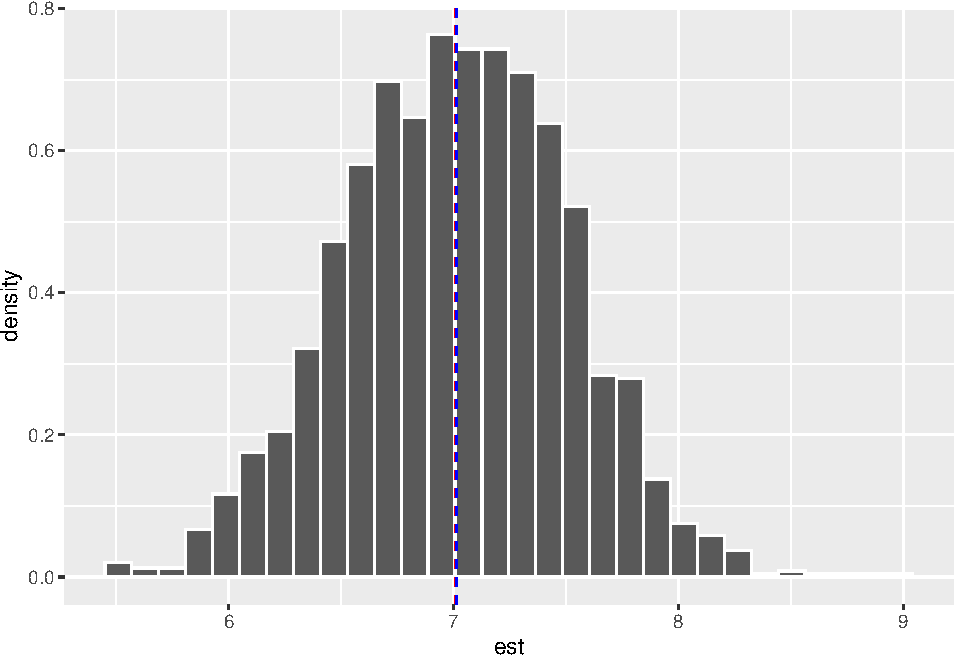
\includegraphics{for_markdown_files/figure-latex/unnamed-chunk-9-1.pdf}

\begin{Shaded}
\begin{Highlighting}[]
\CommentTok{\# Exponential}

\NormalTok{fit2 }\OtherTok{\textless{}{-}} \FunctionTok{lmer}\NormalTok{(DWB100 }\SpecialCharTok{\textasciitilde{}}\NormalTok{ WkDay }\SpecialCharTok{+}\NormalTok{ z2sleep }\SpecialCharTok{+}\NormalTok{ (}\DecValTok{1}\SpecialCharTok{|}\NormalTok{NameID), }\AttributeTok{data =}\NormalTok{ DWBdata)}
\NormalTok{M }\OtherTok{\textless{}{-}} \FloatTok{2e3}
\NormalTok{X }\OtherTok{\textless{}{-}}\NormalTok{ fit2 }\SpecialCharTok{\%\textgreater{}\%} \FunctionTok{model.matrix}\NormalTok{()}
\NormalTok{Z }\OtherTok{\textless{}{-}}\NormalTok{ fit2 }\SpecialCharTok{\%\textgreater{}\%} \FunctionTok{getME}\NormalTok{(}\AttributeTok{name=}\StringTok{"Z"}\NormalTok{)}
\NormalTok{beta }\OtherTok{\textless{}{-}} \FunctionTok{fixef}\NormalTok{(fit2)}
\NormalTok{tau }\OtherTok{\textless{}{-}}\NormalTok{ (}\FunctionTok{VarCorr}\NormalTok{(fit2) }\SpecialCharTok{\%\textgreater{}\%} \FunctionTok{as.data.frame}\NormalTok{())}\SpecialCharTok{$}\NormalTok{sdcor[}\DecValTok{1}\NormalTok{]}
\NormalTok{sigma }\OtherTok{\textless{}{-}}\NormalTok{ (}\FunctionTok{VarCorr}\NormalTok{(fit2) }\SpecialCharTok{\%\textgreater{}\%} \FunctionTok{as.data.frame}\NormalTok{())}\SpecialCharTok{$}\NormalTok{sdcor[}\DecValTok{2}\NormalTok{]}
\NormalTok{resMat }\OtherTok{\textless{}{-}} \FunctionTok{matrix}\NormalTok{(}\ConstantTok{NA}\NormalTok{,M,}\DecValTok{3}\NormalTok{)}
\ControlFlowTok{for}\NormalTok{ (i }\ControlFlowTok{in} \DecValTok{1}\SpecialCharTok{:}\NormalTok{M) \{}
\NormalTok{B }\OtherTok{\textless{}{-}}\NormalTok{ (}\FunctionTok{rexp}\NormalTok{(}\DecValTok{27}\NormalTok{)}\SpecialCharTok{{-}}\DecValTok{1}\NormalTok{)}\SpecialCharTok{*}\NormalTok{tau}
\NormalTok{eps }\OtherTok{\textless{}{-}} \FunctionTok{rnorm}\NormalTok{(}\FunctionTok{nrow}\NormalTok{(DWBdata), }\DecValTok{0}\NormalTok{, sigma)}
\NormalTok{y }\OtherTok{\textless{}{-}}\NormalTok{ X }\SpecialCharTok{\%*\%}\NormalTok{ beta }\SpecialCharTok{+}\NormalTok{ Z }\SpecialCharTok{\%*\%}\NormalTok{ B }\SpecialCharTok{+}\NormalTok{ eps}
\NormalTok{simdata }\OtherTok{\textless{}{-}}\NormalTok{ DWBdata}
\NormalTok{simdata}\SpecialCharTok{$}\NormalTok{y }\OtherTok{\textless{}{-}} \FunctionTok{as.numeric}\NormalTok{(y)}
\NormalTok{lmm }\OtherTok{\textless{}{-}} \FunctionTok{lmer}\NormalTok{(y }\SpecialCharTok{\textasciitilde{}}\NormalTok{ WkDay }\SpecialCharTok{+}\NormalTok{ z2sleep }\SpecialCharTok{+}\NormalTok{ (}\DecValTok{1}\SpecialCharTok{|}\NormalTok{NameID), }\AttributeTok{data =}\NormalTok{ simdata)}
\NormalTok{resMat[i,}\DecValTok{1}\NormalTok{] }\OtherTok{\textless{}{-}} \FunctionTok{fixef}\NormalTok{(lmm)[}\DecValTok{8}\NormalTok{]}
\NormalTok{resMat[i,}\DecValTok{2}\SpecialCharTok{:}\DecValTok{3}\NormalTok{] }\OtherTok{\textless{}{-}} \FunctionTok{confint}\NormalTok{(lmm,}\AttributeTok{method=}\StringTok{"Wald"}\NormalTok{)[}\DecValTok{10}\NormalTok{,]}
\NormalTok{\}}
\NormalTok{resData }\OtherTok{\textless{}{-}} \FunctionTok{data.frame}\NormalTok{(resMat)}
\FunctionTok{names}\NormalTok{(resData) }\OtherTok{\textless{}{-}} \FunctionTok{c}\NormalTok{(}\StringTok{"est"}\NormalTok{,}\StringTok{"lower"}\NormalTok{,}\StringTok{"upper"}\NormalTok{)}
\end{Highlighting}
\end{Shaded}

\begin{Shaded}
\begin{Highlighting}[]
\NormalTok{resData }\SpecialCharTok{\%\textgreater{}\%} \FunctionTok{summarise}\NormalTok{(}\AttributeTok{bias =} \FunctionTok{mean}\NormalTok{(est)}\SpecialCharTok{{-}}\NormalTok{beta[}\StringTok{"z2sleep"}\NormalTok{])}
\end{Highlighting}
\end{Shaded}

\begin{verbatim}
##        bias
## 1 0.0140701
\end{verbatim}

\begin{Shaded}
\begin{Highlighting}[]
\NormalTok{resData }\SpecialCharTok{\%\textgreater{}\%} \FunctionTok{mutate}\NormalTok{(}\AttributeTok{cover =}\NormalTok{ (beta[}\DecValTok{8}\NormalTok{] }\SpecialCharTok{\textgreater{}}\NormalTok{ lower)}\SpecialCharTok{*}\NormalTok{(beta[}\DecValTok{8}\NormalTok{] }\SpecialCharTok{\textless{}}\NormalTok{ upper)) }\SpecialCharTok{\%\textgreater{}\%} \FunctionTok{summarise}\NormalTok{(}\AttributeTok{coverage =} \FunctionTok{mean}\NormalTok{(cover))}
\end{Highlighting}
\end{Shaded}

\begin{verbatim}
##   coverage
## 1    0.949
\end{verbatim}

\begin{Shaded}
\begin{Highlighting}[]
\FunctionTok{ggplot}\NormalTok{() }\SpecialCharTok{+}
\FunctionTok{geom\_histogram}\NormalTok{(resData, }\AttributeTok{mapping =} \FunctionTok{aes}\NormalTok{(}\AttributeTok{x =}\NormalTok{ est, }\AttributeTok{y =}\NormalTok{ ..density..), }\AttributeTok{color =} \StringTok{"white"}\NormalTok{, }\AttributeTok{bins =} \DecValTok{30}\NormalTok{) }\SpecialCharTok{+}
\FunctionTok{geom\_vline}\NormalTok{(}\AttributeTok{xintercept =}\NormalTok{ beta[}\DecValTok{8}\NormalTok{], }\AttributeTok{color =} \StringTok{"red"}\NormalTok{, }\AttributeTok{linetype =} \StringTok{"dashed"}\NormalTok{) }\SpecialCharTok{+}
\FunctionTok{geom\_vline}\NormalTok{(}\AttributeTok{xintercept =} \FunctionTok{mean}\NormalTok{(resData}\SpecialCharTok{$}\NormalTok{est), }\AttributeTok{color =} \StringTok{"blue"}\NormalTok{, }\AttributeTok{linetype =} \StringTok{"dashed"}\NormalTok{)}
\end{Highlighting}
\end{Shaded}

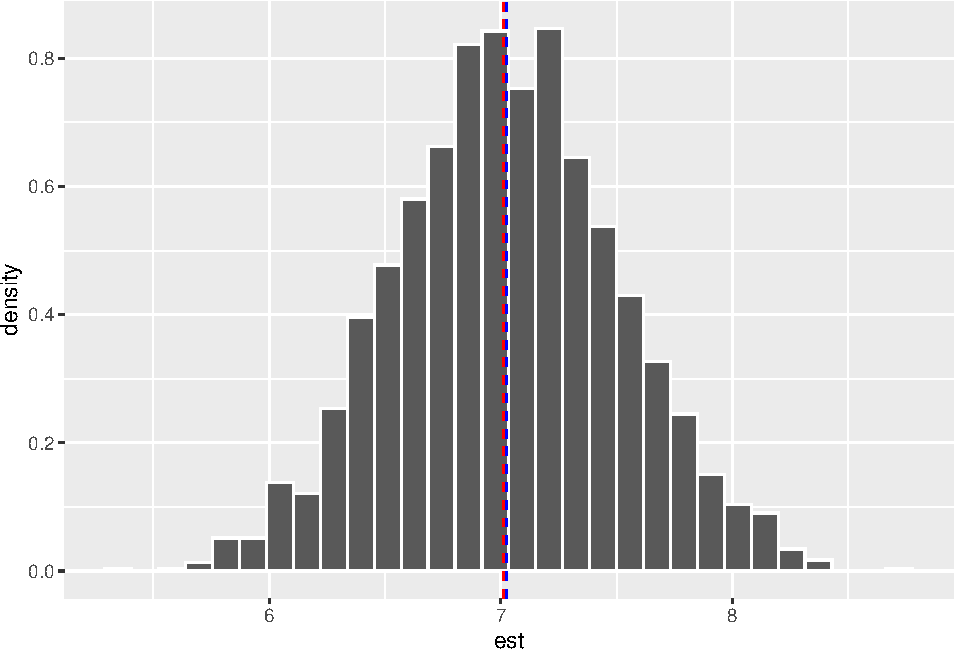
\includegraphics{for_markdown_files/figure-latex/unnamed-chunk-13-1.pdf}

\end{document}
